
\documentclass[11pt]{article}
\usepackage[margin=1in]{geometry}

%Set up packages
\usepackage{amsmath,amssymb,amsthm}
\usepackage{graphicx}
\usepackage{subcaption}
\usepackage{textcomp, gensymb}
\usepackage{float}
\usepackage{pdfpages}
\usepackage[hidelinks]{hyperref}
\usepackage{listings}
\usepackage{cancel}
\usepackage{subcaption}
\usepackage{caption}
\usepackage{tabularx}

\usepackage{mdframed}
\usepackage{grffile}

\newcommand{\bm}{\boldsymbol}
\newcommand{\bI}{\mathbb{I}}
\newcommand{\bR}{\mathbb{R}}

\setlength\parindent{0pt}

\title{\bf Supersonic Flow Over a Diamond Airfoil}
\author{Group 2 : Andrew Doty, Buck Newberry, Andres Suniaga, David Valenzano \\[2mm] \textit{Dept. of Aerospace Engineering and Engineering Mechanics, The University of Texas at Austin}}
\date{November 19, 2024}

\begin{document}
\maketitle

% \noindent\makebox[\textwidth]{\rule{\textwidth}{0.2pt}}
% \tableofcontents
% \noindent\makebox[\textwidth]{\rule{\textwidth}{0.2pt}}

\textbf{Abstract} This experiment intends to compare experimental data from supersonic flow over a diamond-shaped airfoil with predictions from shock-expansion theory. Tests were conducted on a diamond profile at Machs $2.0, 2.25, 2.5,$ and $3.0$ across different angles of attack $0\degree, 3\degree,$ and $7\degree$. The findings show discrepancies from theory as the expansions and recompression shocks occurred much more upstream with our test model. Experimental results show notable deviations in $C_{L}$, $C_{D}$, and the center of pressure locations, $x_{\text{cp}}$ and $y_{\text{cp}}$, from theoretical values. Discrepancies can be attributed to the non-ideal geometry of the test article, particularly the blunted edges as opposed to the sharp corners shown in theory, and perturbations in the supposed angles of attack of the model in the flow. These factors provide critical sources of error in the experimental design.

\pagebreak

\section{Introduction}
%Relate to historic and current work based on references, plus what this report is about with relation to previous research
Diamond-shaped airfoils often appear in works related to supersonic flow. Reports on this subject go as far back as the 1950s with a paper published in 1953 about reducing the effects of icing on aircraft and missiles through experiments with double-wedged and diamond-shaped airfoils at transonic and supersonic flow.$^\text{\hyperlink{reference}{4}}$ This particular paper discusses the analytical study of impingement of water droplets on wedge and diamond-shaped airfoils at supersonic speeds, which is an example of how the experiment discussed in our report can be advanced.
\vspace{3mm}

A bit further in time, a paper published in 1959 by NASA discusses the design of a diamond-shaped wing and body combination to find the minimum wave drag at sonic condition, which was consistent with the decreasing supersonic wave-drag coefficient.$^\text{\hyperlink{reference}{5}}$ Tests were conducted in a range of Mach numbers from $0.2$ to $3.50$ at Reynolds numbers based around the M.A.C. of $6\times 10^{6}$ to $9\times 10^{6}$. Comparisons were made with a minimum wave-drag body such as the Sears-Haack body and with theoretical predictions. There was a gradual decrease in wave drag from sonic conditions up to $M=1.2$, but beyond that there was a rise in wave-drag. This discrepancy was attributed to part of the body contouring and the wing geometry, similar to our sources of error.
\vspace{3mm}

Moving ahead in time to 1974, another NASA document, very similar to our experiment, is written to compare two-dimensional shock-expansion theory with experiments on delta-planform wings at supersonic speeds.$^\text{\hyperlink{reference}{1}}$ Particularly, this paper is interested in optimizing airfoil design for supersonic flow. Their experiments used four delta-planform wings with a leading edge sweep, $\Lambda_{\text{LE}} = 65\degree$, and very thin modified diamond airfoils with a thickness-to-chord ratio, $\frac{t}{c} = 0.06$. Unlike our findings, results of drag polars and lift as a function of angle of attack for this experiment showed very close resemblance to theoretical values. It is noted that theory underestimated lift with a difference increasing with angle of attack. However, the experiment found excellent agreement with picthing-moment coefficients. 
\vspace{3mm}

Delta wings were further discussed in a NASA report published in 1988 concerning their aerodynamics at supersonic speeds.$^\text{\hyperlink{reference}{3}}$ This report was a combined experimental and theoretical study intended to provide a better understanding of the effects of airfoil profile, wing sweep, and Mach number on delta wing aerodynamics in supersonic flow. The diamond-shaped airfoil showed a reduction in wave-drag compared to circular arc and four-digit series airfoils. This study is another example of how our experiment can be extended to compare to other profiles.
\vspace{3mm}

A more current publication in 2020 studies the effects of large-amplitude step motion on diamond-shaped airfoils in supersonic flow.$^\text{\hyperlink{reference}{2}}$ This paper concerns unsteady aerodynamics as it discusses how aerodynamic forces evolve with a sudden change in angle of attack. The objective of this experiment was to develop theoretical models to describe wave speed, pressure, and force in distinct flow regions of this diamond-shaped profile system. This study traces back to Heaslet and Lomax who wrote a paper back in 1949 on unsteady lift of 2-Dimensional airfoils in supersonic flow.$^\text{\hyperlink{reference}{6}}$ This shows how extensive an experiment can go.
\vspace{3mm}

These previous works build off of the simple experiment our paper entails to more specific applications for aircraft and high-speed aerodynamics. In this report, we detail our experimental findings of supersonic flow over a diamond airfoil from Machs $2.0$ to $3.0$ at different angles of attack $0\degree, 3\degree,$ and $7\degree$. Flow visualizations and data gathered from the experiment are then compared to that of shock-expansion theory to observe how well this experiment satisfies theoertical predictions.

\pagebreak

\section{Theory}
The basis for this report is the Schlieren imaging technique that takes advantage of the normally imperceptible changes in the index of refraction of gases that occur due to changes in destiny. Light from a point source is reflected and made parallel by a concave parabolic mirror. This light passes through a section of air and refracted light is disturbed from its straight path. Half of this disturbed light is blocked by a razors edge before it reaches a camera. The resulting image has the disturbed light showing up as brighter spots where it converges and darker spots where it has been diverged away from. This results in the image displaying the changes in the air's density like in the shocks and expansion fans in this report. 
\vspace{2.5mm}

Similarly important are the relations of shocks. If a compressible gas moves around an object, for low subsonic Mach numbers, it will simply flow around it. However, if that flow is going faster than the speed of sound and the change in properties like area are rapid, then a shock is formed. These changes in flow properties are non-isentropic as the changes in temperature and velocity are large within the shock itself. The specific relation used in this report are the oblique shock relations shown below:

\begin{equation*}
    \tan{(\theta)} = 2\cot{(\beta)}\dfrac{M_{1}^{2} \sin^{2}{(\beta)} - 1}{M_{1}^{2}(\gamma + \cos{(2\beta)}) + 2}
\end{equation*}
\vspace{2.5mm}

The $\theta$-$\beta$-$\text{Mach}$ relation for predicting the wave angle $\beta$ the shock will form at a given incoming Mach number $M_{1}$ and turn angle the flow is making $\theta$.

\begin{equation*}
    M_{1_{\text{N}}} = M_{1} \sin{(\beta)}
\end{equation*}

\begin{equation*}
    M_{2_{\text{N}}}^{2} = \dfrac{1 + \left(\dfrac{\gamma-1}{2}\right) M_{1_{\text{N}}}^{2}}{\gamma M^{2}_{1_{\text{N}}} - \left(\dfrac{\gamma-1}{2}\right)}
\end{equation*}

\begin{equation*}
    M_{2} = \dfrac{M_{2_{\text{N}}}}{\sin{(\beta - \theta)}}
\end{equation*}

The normal shock relation is used with the assumption that the change in Mach number across the shock only occurs to the normal portion of the flow. This is used to predict the post-shock Mach number $M_{2}$ given an incoming Mach number $M_{1}$ across an oblique shock. The change in static pressure across the shock is modeled by:

\begin{equation*}
    P_{2} = P_{1}\left[1 + \left(\dfrac{2\gamma}{\gamma + 1}\right) (M^{2}_{1_{\text{N}}} - 1)\right]
\end{equation*}

Where $P_{1}$ is the freestream static pressure before the shock and $P_{2}$ being the post shock static pressure.
\vspace{5mm}

Following the shock on the diamond airfoils will be a Prandtl-Meyer expansion fan for the flow going over the middle section of the diamond. The flow has to turn into and expand around an angle $\theta$ and the relation of the pre and post-fan Mach number is given by:

\begin{equation*}
    \theta = \nu(M_{2}) - \nu(M_{1})
\end{equation*}

\begin{equation*}
    \nu = \sqrt{\dfrac{\gamma + 1}{\gamma - 1}}\tan^{-1}{\left( \sqrt{\dfrac{\gamma-1}{\gamma+1}} (M^{2} - 1)   \right)} - \tan^{-1}{(\sqrt{M^{2} - 1})}
\end{equation*}

Where $\nu$ is a function of the flow's Mach number. The resulting Mach number can then give us the post-turn static pressure through the isentropic relations that connect a flow's Mach number to its properties since Prandtl-Meyer fans are isentropic and thus the stagnation properties are constant through the fan.

\begin{equation*}
    P_{0_{1}} = P_{1}\left[1 + (\dfrac{\gamma -1}{2}) M_{1}^{2} \right] ^{\frac{\gamma}{\gamma - 1}} = P_{0_{2}}
\end{equation*}

\begin{equation*}
    P_{2} = \dfrac{P_{0_{2}}}{\left[1 + (\dfrac{\gamma -1}{2}) M_{2}^{2} \right] ^{\frac{\gamma}{\gamma - 1}}}
\end{equation*}

The coefficients of sectional lift and drag are found from distributions of pressure across the 4 faces of the diamond to ascertain some lift and drag forces and then combined with the standard expressions of lift and drag:

\begin{equation*}
    l = \frac{1}{2}\rho_{\infty}U_{\infty}^{2}C_{l}c
\end{equation*}

\begin{equation*}
    d = \frac{1}{2}\rho_{\infty}U_{\infty}^{2}C_{d}c
\end{equation*}

Which then turn into:

\begin{equation*}
    C_{l} = \dfrac{1}{\gamma P_{\infty} M_{\infty}^{2} \cos{(\theta)}} \left[(P_{3} - P_{2})\cos{(\theta + \alpha)} + (P_{4}-P_{1})\cos{(\theta-\alpha)}\right]
\end{equation*}

\begin{equation*}
    C_{d} = \dfrac{1}{\gamma P_{\infty} M_{\infty}^{2} \cos{(\theta)}} \left[(P_{1} - P_{4})\sin{(\theta - \alpha)} + (P_{3} - P_{2})\sin{(\theta + \alpha)}\right]
\end{equation*}

Derivations of which can be found in the appendix of this report.$^{\hyperlink{derivations}{\text{A}}}$
\vspace{5mm}

The center of pressure for the airfoil are determined by:
\begin{equation*}
    \dfrac{CP_{x}}{c} = \dfrac{\frac{1}{4}(P_{1}-P_{3}) + \frac{3}{4}(P_{2} - P_{4})}{P_{1} - P_{3} + P_{2} - P_{4}}
\end{equation*}

\begin{center}
    if $\alpha = 0\degree \implies$ \(\left|\dfrac{CP_{x}}{c}\right|_{\alpha = 0\degree} = \dfrac{\frac{1}{4}P_{1} + \frac{3}{4}P_{2}}{P_{1} + P_{2}}\)
\end{center}

\begin{equation*}
    \dfrac{CP_{y}}{t} = \dfrac{P_{1} - P_{2} - P_{3} + P_{4}}{2(P_{1} - P_{2} + P_{3} - P_{4}}
\end{equation*}
\vspace{2.5mm}

Where the static pressures of the faces are:

\begin{figure}[H]
    \centering
    \includegraphics[width = 0.75\linewidth]{ReportImages/DiamondAirfoilSurfacePressures.png}
\end{figure}
\pagebreak

\section{Experimental Setup}

The experiment was conducted using the Aerolab Variable Mach Number Wind Tunnel, capable of producing supersonic flows with Mach numbers ranging from approximately 2.25 to 3. The test section of the wind tunnel is nominally 3" * 3". A diamond airfoil model with four pressure transducers was mounted in the test section at a $0^\circ$ angle of attack, and ran at 3 mach numbers with 3 angles of attack. The experimental setup is shown in Figure \ref{fig:lab3_setup}.

\begin{figure}[H]
    \centering
    \includegraphics[width=0.8\textwidth]{ReportImages/experimental-setup.png}
    \caption{Experimental setup for Lab 3: Supersonic Flow over a Diamond Airfoil}
    \label{fig:lab3_setup}
\end{figure}


\begin{table}[H]
    \centering
    \caption{Schlieren System Components and Functions}
    \renewcommand{\arraystretch}{1.5} % Adjust row height
    \begin{tabularx}{\textwidth}{|p{3.5cm}|X|} % Use X for flexible width
    \hline
    \textbf{Component} & \textbf{Function} \\
    \hline
    Pulsed Light Source & Provides high-intensity, short-duration illumination for capturing instantaneous flow features. \\
    \hline
    Pin hole & Acts as a spatial filter to create a point source of light, improving image quality by reducing diffuse light. \\
    \hline
    Color filter & Optional component that can be used to produce color Schlieren images or filter specific wavelengths. \\
    \hline
    Concave Mirror 1 & Collimates the light beam from the point source into parallel rays that pass through the test section. \\
    \hline
    Dummy mirror & Redirects the light path to create a folded system, reducing the overall space requirements. \\
    \hline
    Test Section & Contains the flow and model being studied, where density gradients cause light ray deflection. \\
    \hline
    Concave Mirror 2 & Focuses the parallel light rays after they pass through the test section. \\
    \hline
    Knife Edge & Blocks a portion of the refracted light rays to create contrast in the final image based on density gradients. \\
    \hline
    Camera & Records the resulting Schlieren image showing flow features. \\
    \hline
    PT (Pressure Transducer) & Measures pressure at various points in the flow field. \\
    \hline
    DAQ (Data Acquisition) & Collects and digitizes pressure measurements from the transducers. \\
    \hline
    PC & Controls data acquisition and image capture, stores experimental data. \\
    \hline
    \end{tabularx}
    \label{tab:schlieren_components}
\end{table}

\subsection{Data Acquisition}

Pressure measurements were recorded using a LabVIEW-based data acquisition system with six pressure transducers.

The pressure data was recorded in volts (gauge pressure) and later converted to appropriate units using calibration constants 15psi/0.1V and 60psi/0.1V.

\subsection{Experimental Procedure}

The experiment followed these steps for each run:

\begin{enumerate}
    \item The wind tunnel was started in the sequence: power, hydraulic, then run.
    \item The initial Mach number was set to a given value and angle of attack was set to 1 of 3 values at that mach number.
    \item Since the pressure transducers had problems, we instead focused on flow visualization using vertical Schlieren.
    \item The wind tunnel was operated only while the run button was held, and shut down in the reverse order of startup once the airflow stopped.
    \item Mach number was adjusted by changing the area ratio and chamber pressure according to the manufacturer's specifications, referencing the "Approximate Minimum Stagnation Pressure vs Mach Number" chart.
    \item The angle of attack was adjusted by adjusting the angle of the diamond airfoil. In post the images were corrected for distortion and mirrored over the y-axis to have a positive angle of attack pointing upwards.
\end{enumerate}

Care was taken to monitor the pressure of the compressed air tank to ensure consistent flow quality across all runs. The experiment was repeated for all mach numbers and angles of attack.


\section{Results \& Discussion}

\subsection{Flow Images}
\begin{figure}[H]
    \centering
    \begin{subfigure}{0.475\linewidth}
        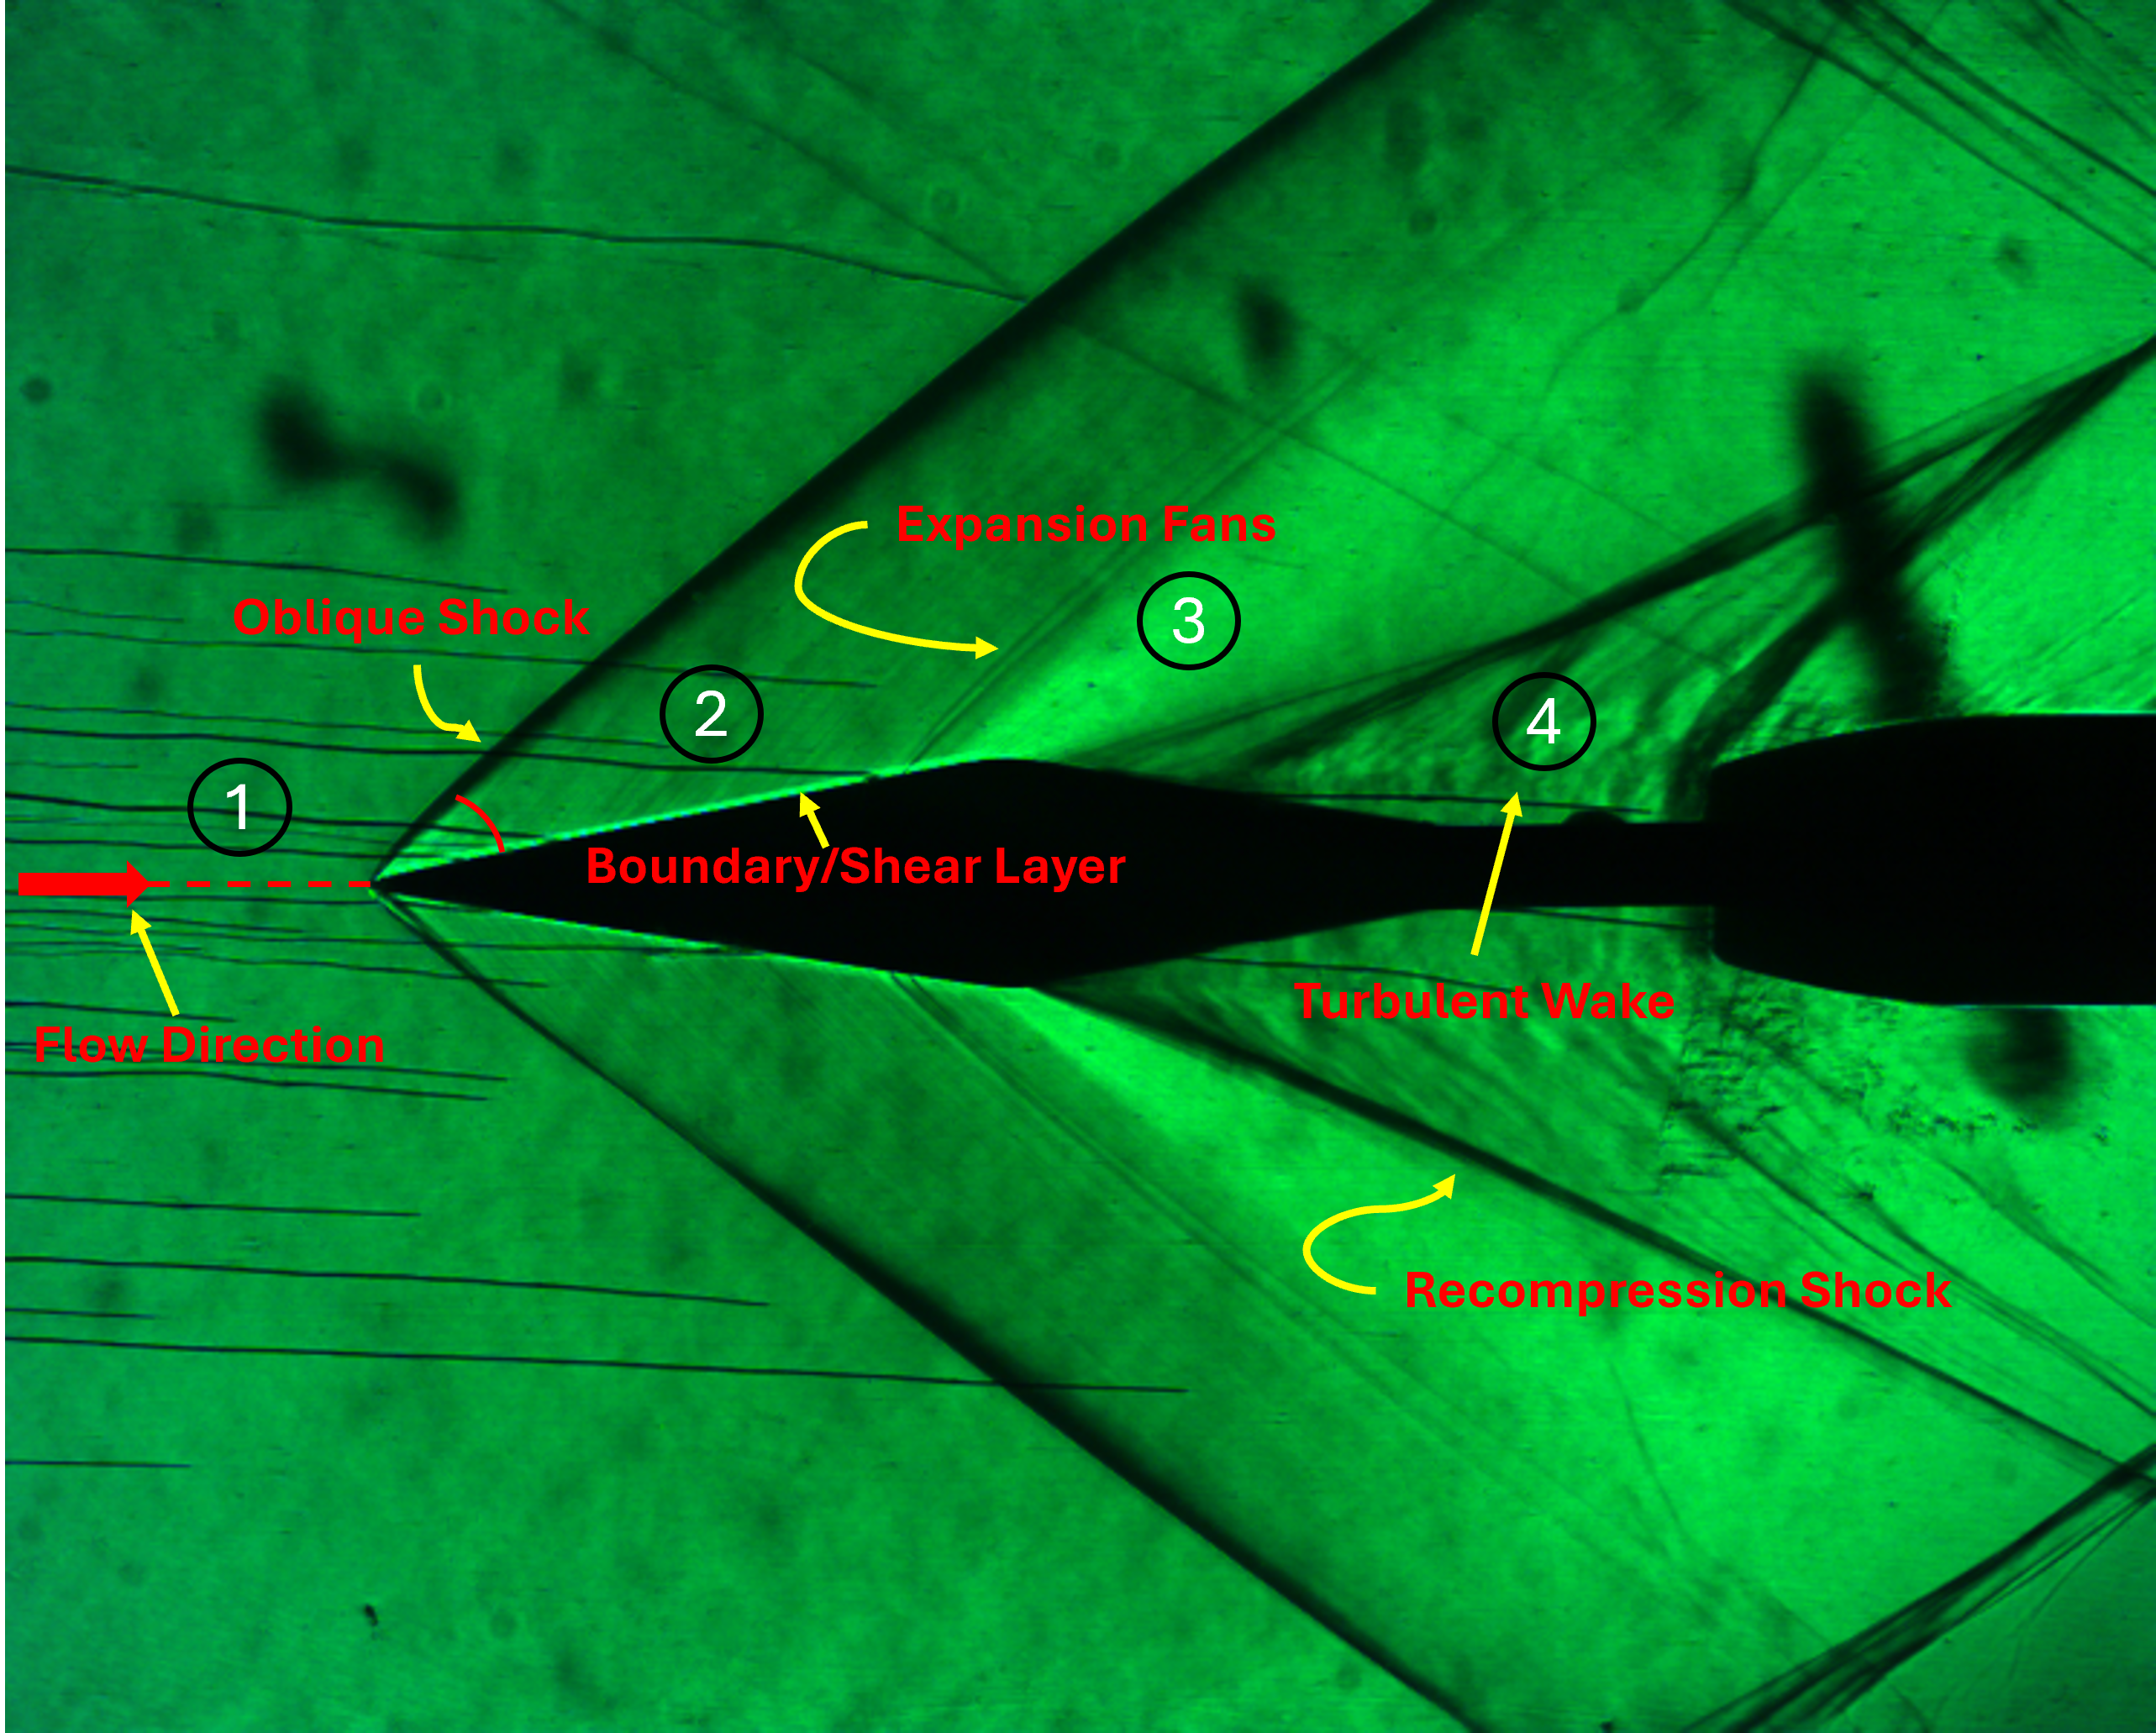
\includegraphics[width = \linewidth]{LabeledImages/Mach2_AoA0.png}
        \caption{Mach 2 flow at $0^\circ$ angle of attack}
        \label{fig:Mach2_AoA0}
    \end{subfigure}
    \hspace{2.5mm}
    \begin{subfigure}{0.475\linewidth}
        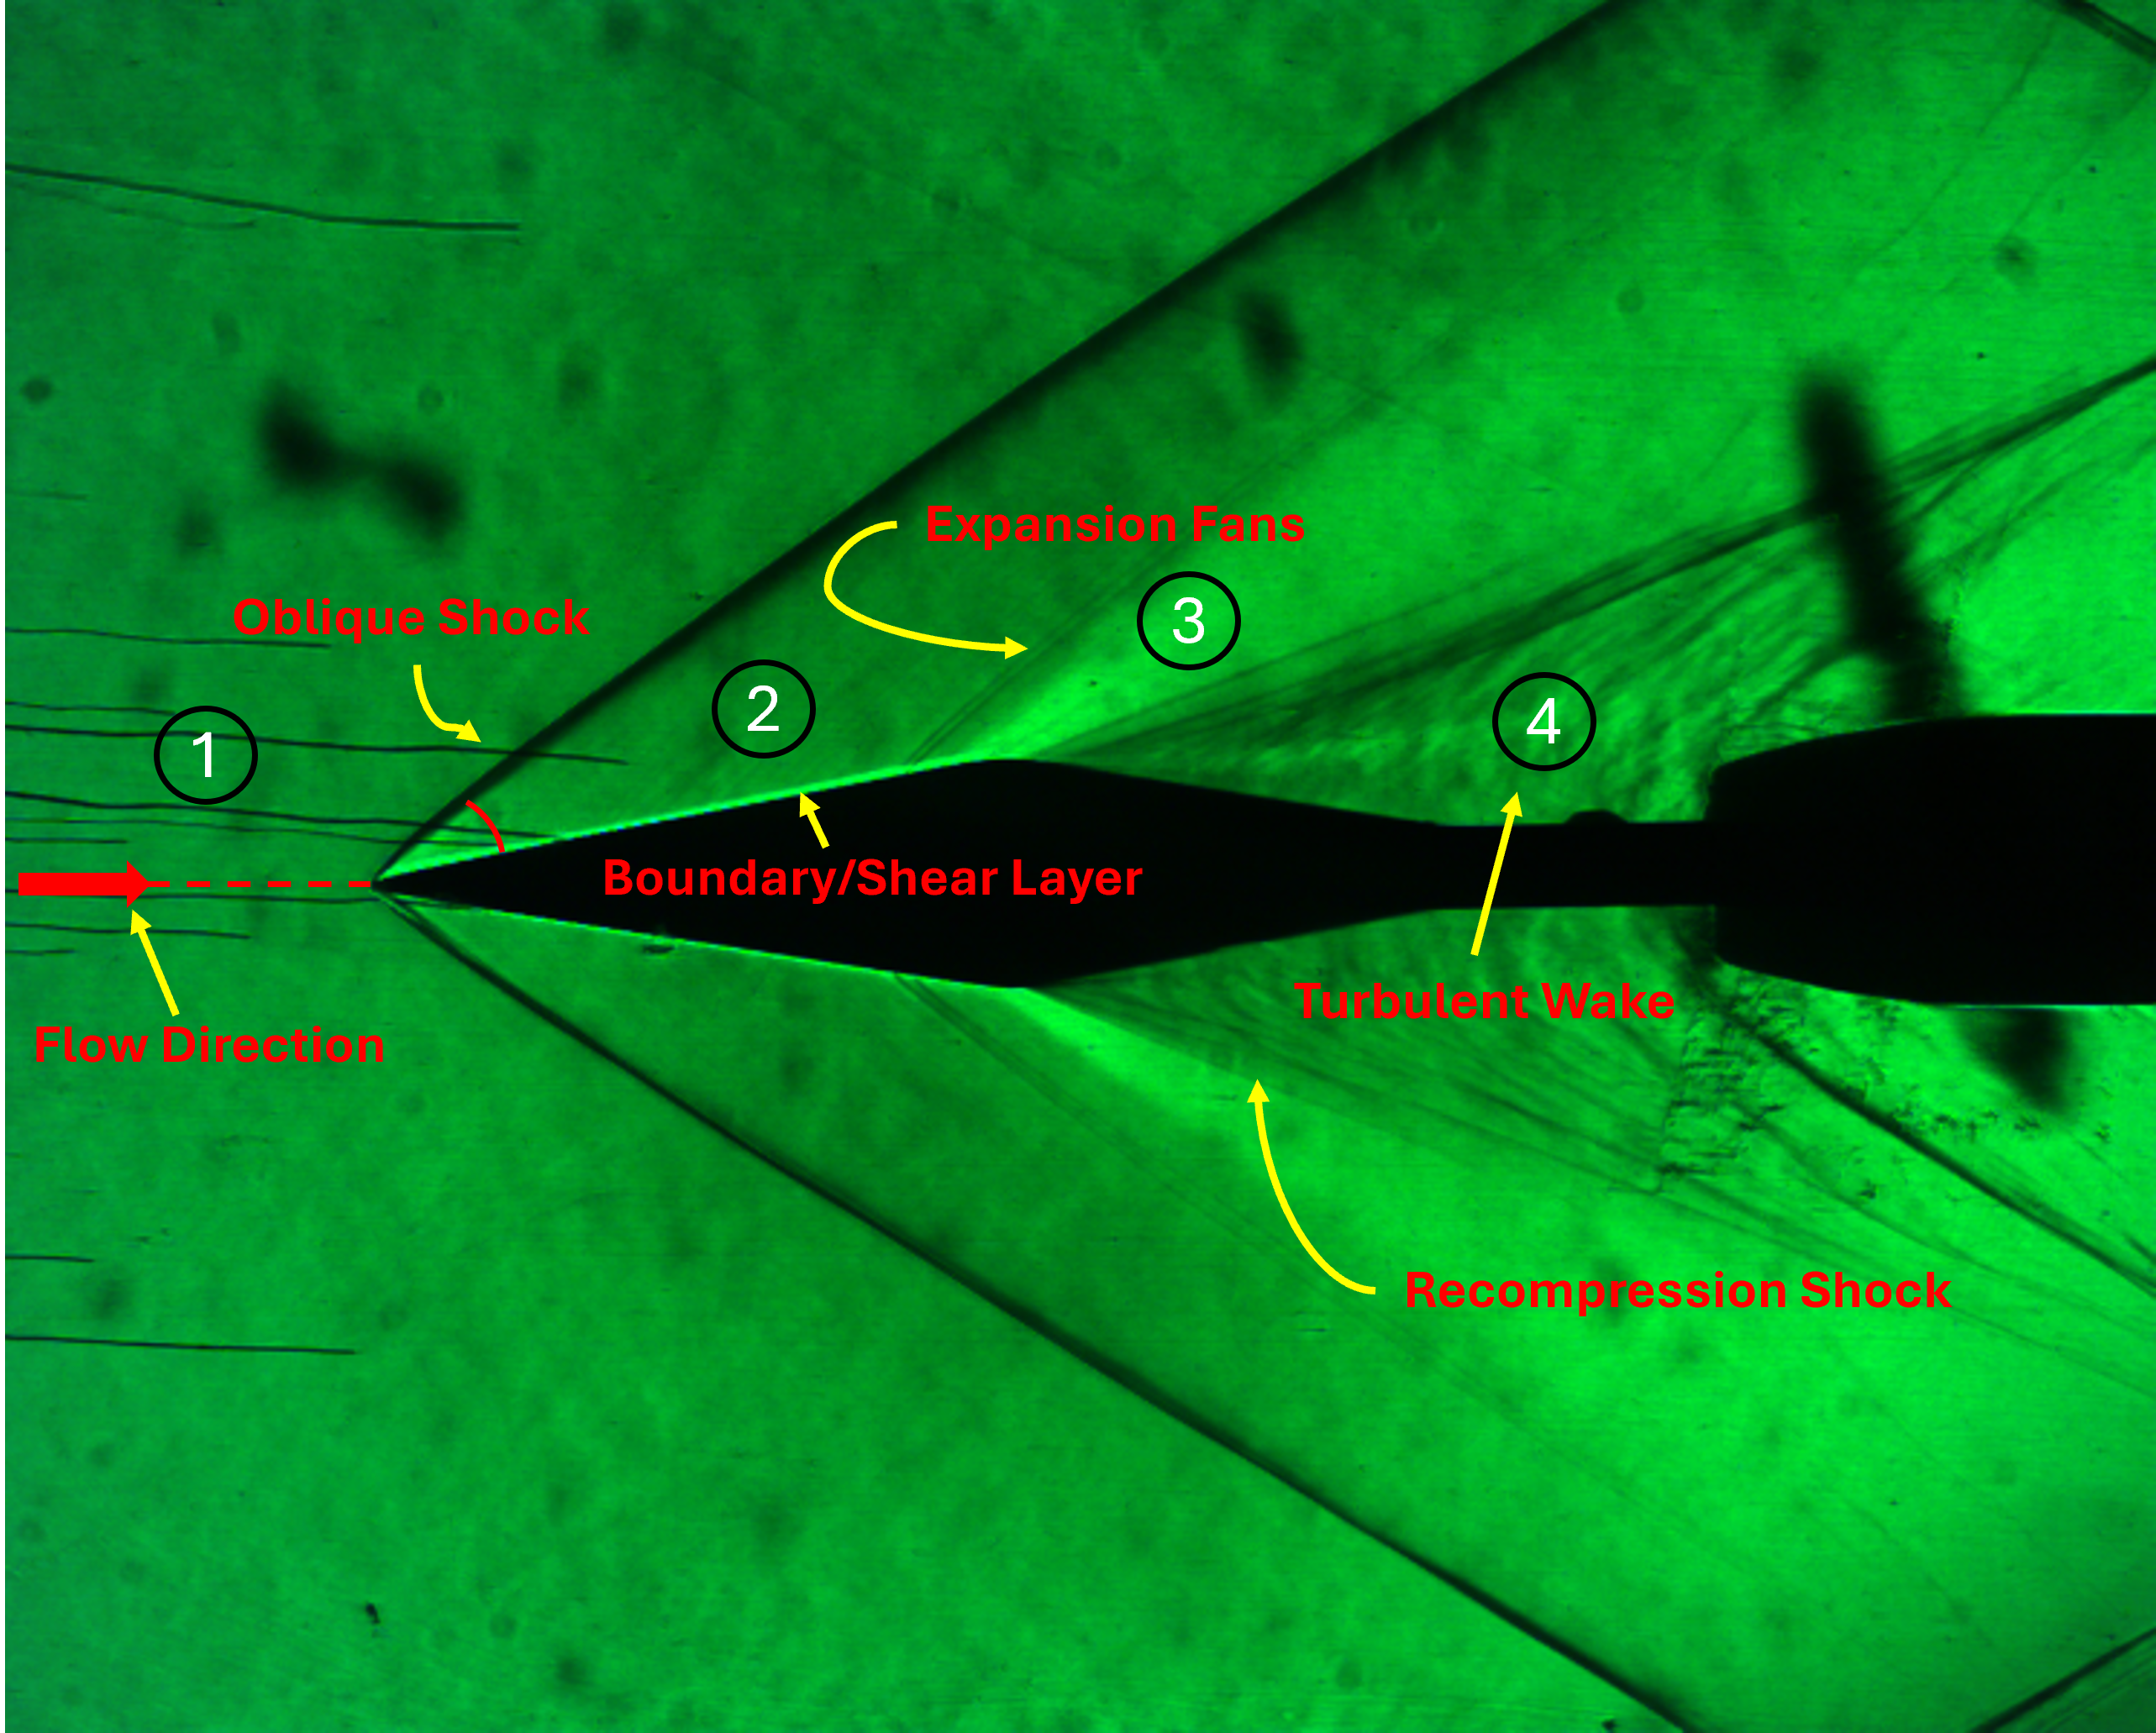
\includegraphics[width = \linewidth]{LabeledImages/Mach25_AoA0.png}
        \caption{Mach 2.5 flow at $0^\circ$ angle of attack}
        \label{fig:Mach25_AoA0}
    \end{subfigure}
    \par\bigskip
    \begin{subfigure}{0.60\linewidth}
        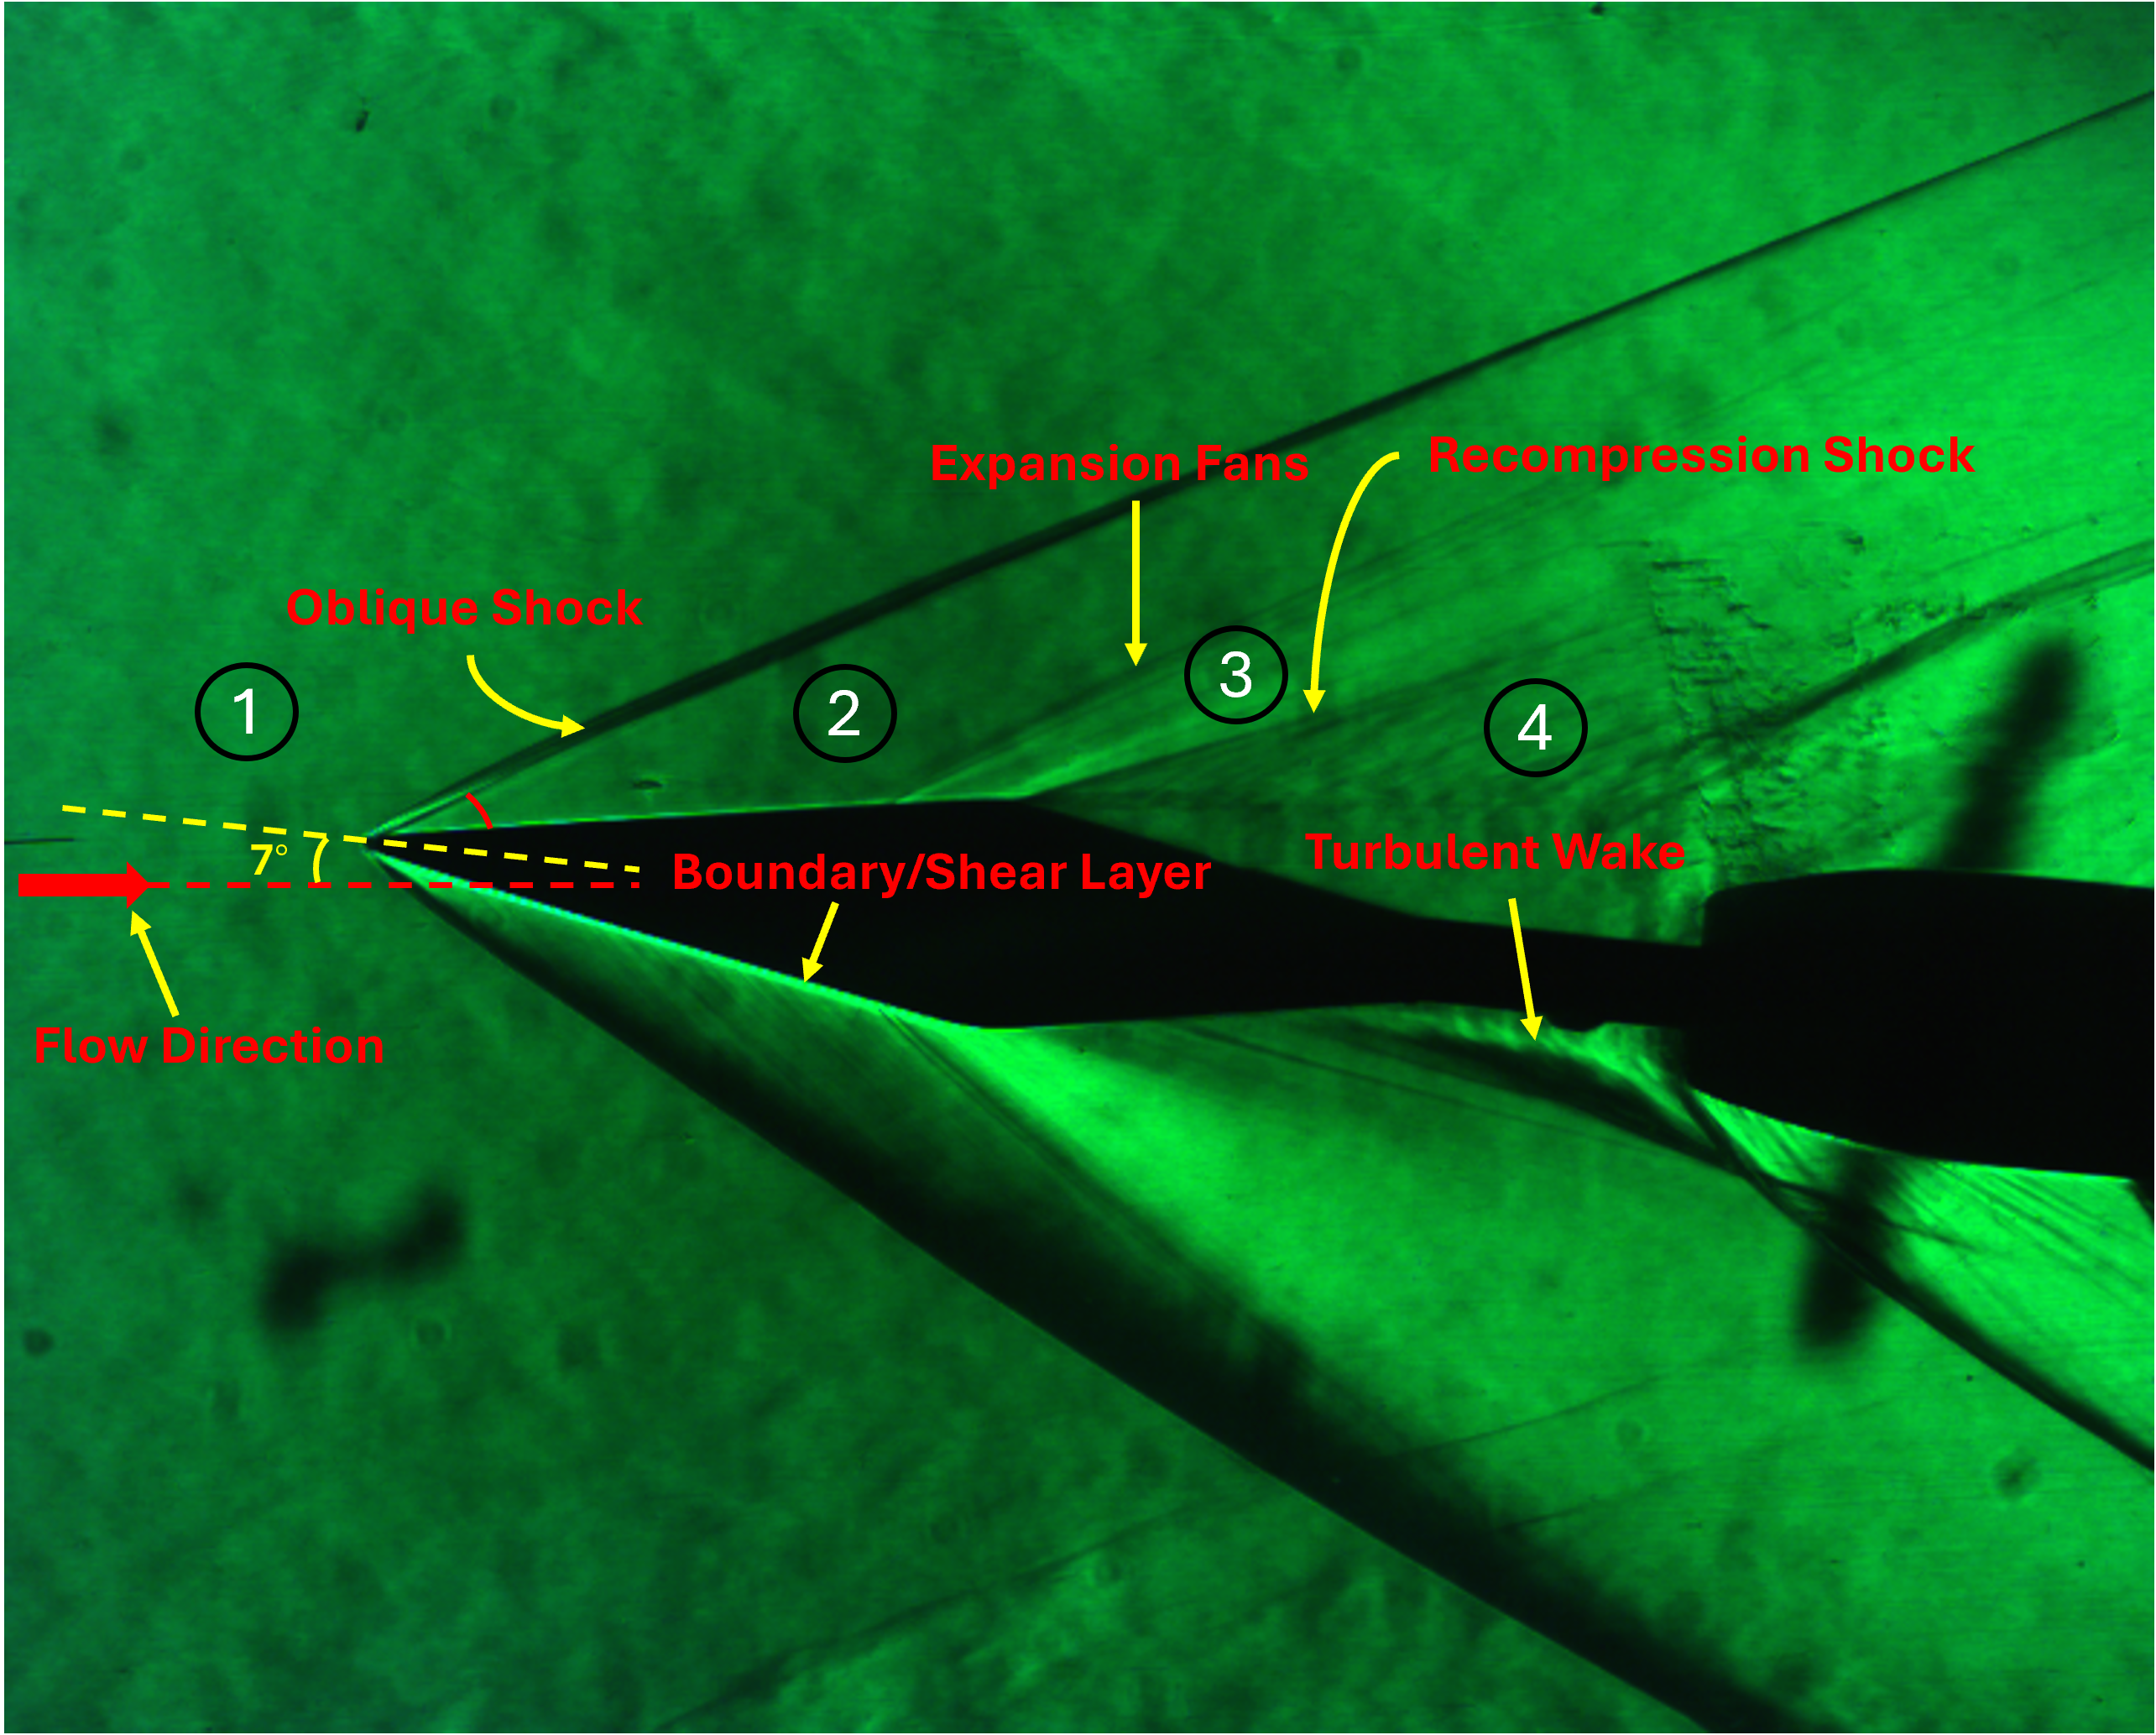
\includegraphics[width=\linewidth]{LabeledImages/Mach3_AoA7.png}
        \caption{Mach 3 flow at $7^\circ$ angle of attack}
        \label{fig:Mach3_AoA7}
    \end{subfigure}
    \caption{Diamond Airfoil at different Mach numbers and angles of attack}
    \label{fig:flow-images}
\end{figure}

Similarities and Differences between the different flows in the above images: 
\begin{itemize}
    \item Similarities:
    \begin{itemize}
        \item Each flow was visualized using a Vertical Schlieren setup.
        \item The density gradients past the shocks and expansions are visibly clear. The density increase across the shock and density drop across the P-M fans are shown clearly by the light captured from the images.
        \item In each image, there is a visible turbulent wake at the end of the diamond airfoil (zone 4).
        \item In each image, the expansion fans and recompression shocks seem to be occurring earlier than on a theoretical diamond airfoil. This discrepancy may be due to the test article not having sharp edges.
        \item Unlabeled: At the bottom of images (a) and (b) in the images, a wave reflection can be seen as the shock interacts with the wall enclosing the test section.
    \end{itemize}
    \vspace{10mm}

    \item Differences:
    \begin{itemize}
        \item Between the Mach 2 and Mach 2.5 flows at $0\degree$ angle of attack, you can clearly see the shock angle becoming smaller. In addition, the expansion zone is smaller too.
        \item At Mach 3 and $7\degree$ angle of attack the boundary layer and expansion zone are much tighter on the top of the diamond (top in reference to image; originally the diamond airfoil was tilted $7\degree$ counterclockwise).
        \item The density gradient is much clearer and bigger on the bottom of the diamond airfoil at $7\degree$ angle of attack in Mach 3 flow. More of the flow is hitting that area.
    \end{itemize}
\end{itemize}

As Mach number increases, the shock wave angle decreases (refer to $\theta$-$\beta$-$M$ Relation). These images satisfy shock-expansion theory in this regard. However, as noted previously, the P-M expansion fans and recompression shocks occur much more upstream than shown on a theoretical diamond airfoil.

\subsubsection{Image Correction}
\begin{figure}[H]
    \centering
    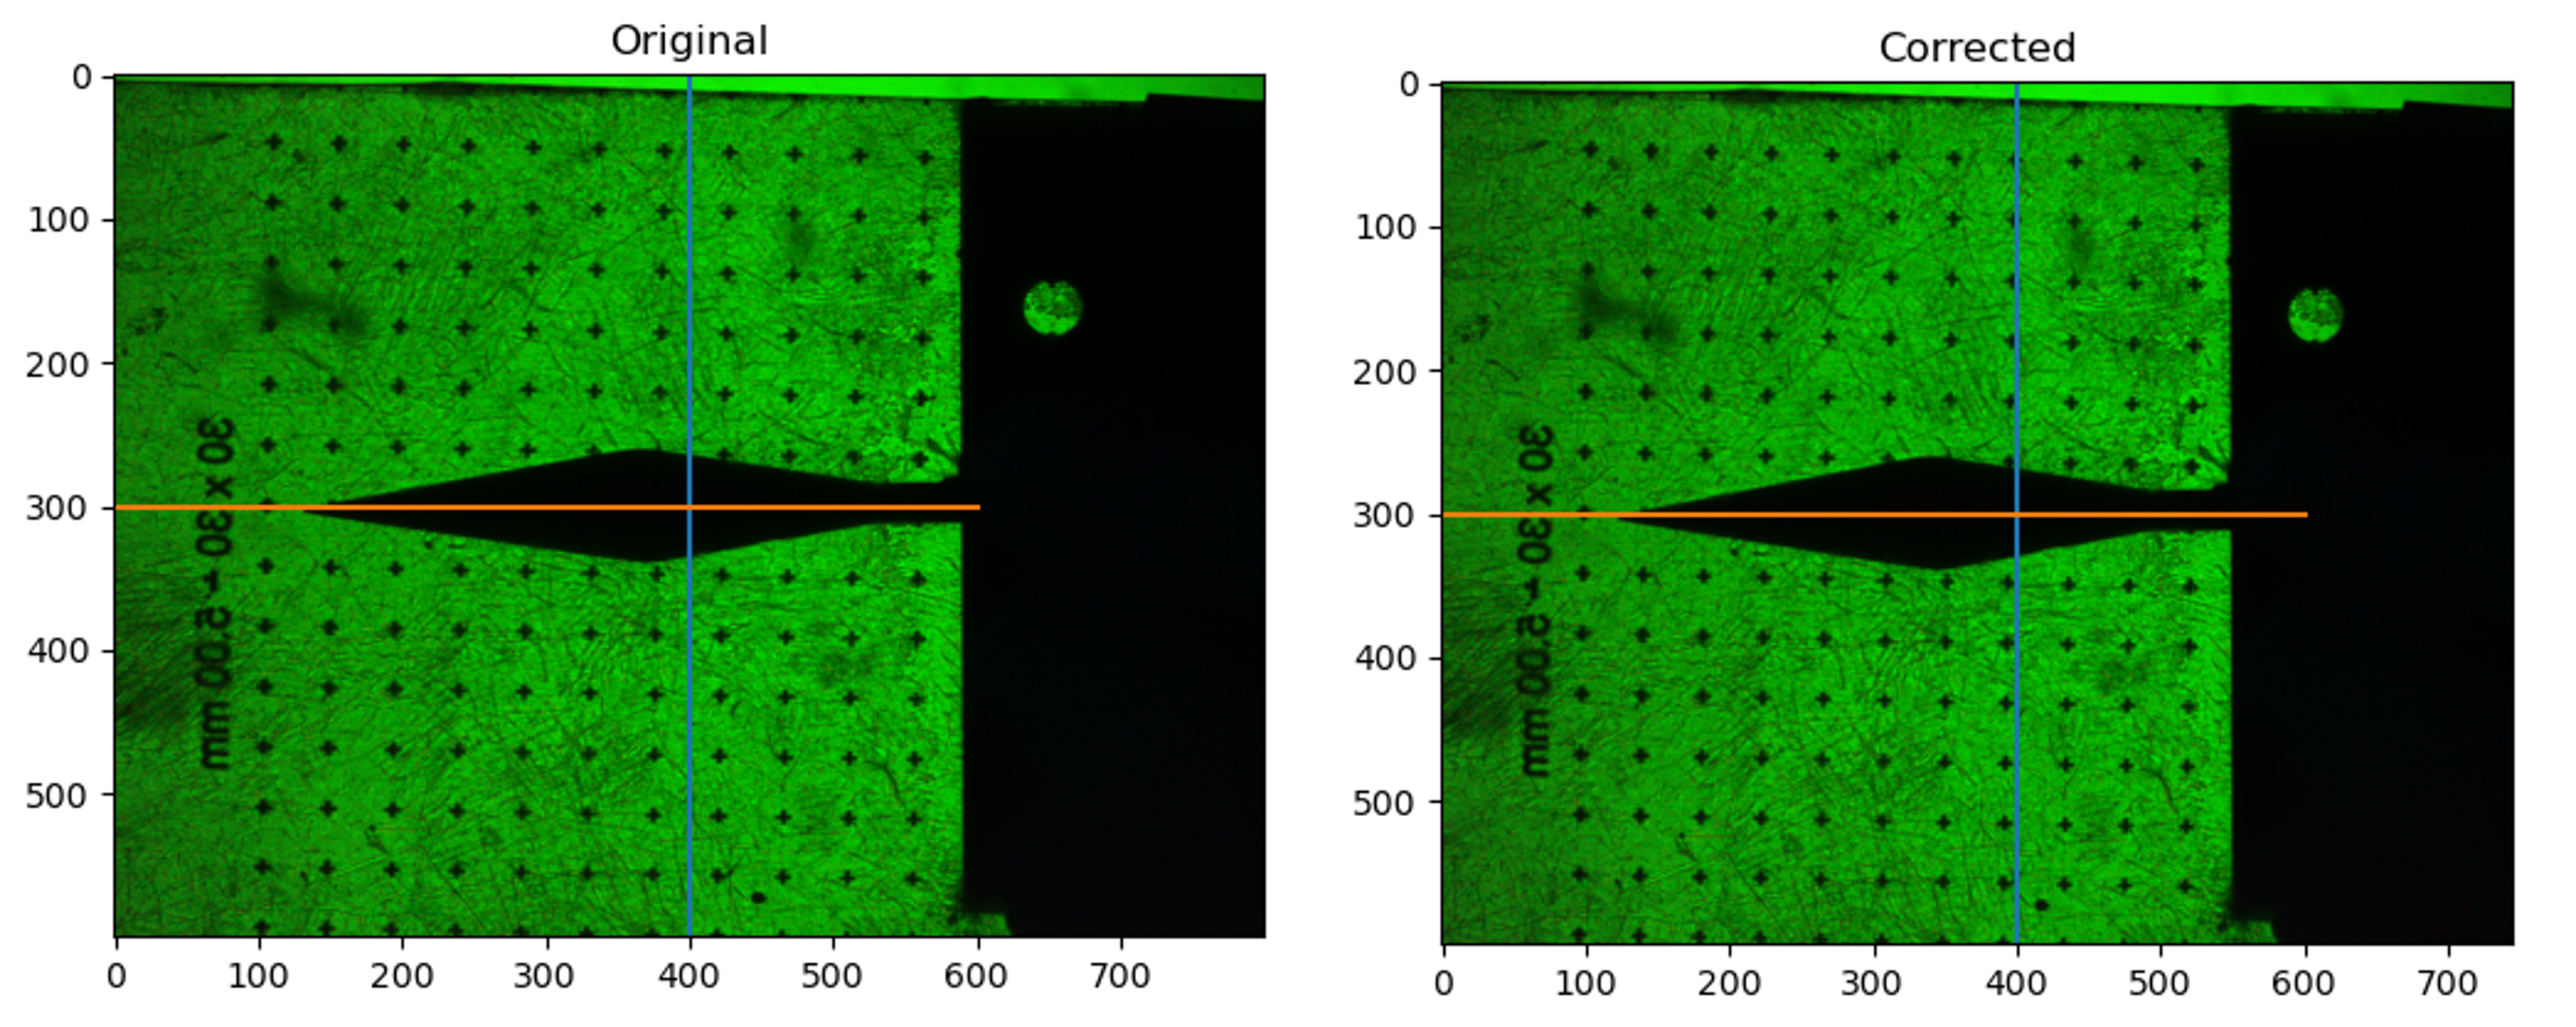
\includegraphics[width = \linewidth]{CorrectedImages/Diamond_GridImage_corrected_vs_raw.png}
    \caption{Corrected wind-off grid image, Raw vs Corrected}
    \label{fig:correction}
\end{figure}

The distortion is not very noticable, however we had to correct for a stretch in the horizontal direction as seen in the images of Figure \ref{fig:correction} and \ref{fig:correctionexample}.
\vspace{5mm}

The raw resolution used was $800$ x $600$ pixels. After correction this became $745$ x $600$ pixels.
\vspace{2.5mm}

A calibration factor was calculated using this formula:
\begin{equation*}
    f = \dfrac{d_{\text{px}}}{n\cdot (5)}
\end{equation*}

The distance between each grid point is $5\, \text{mm}$ and $10$ grid points were used to measure the pixel distance along the grid making $n = 10$. It was found that $f_{x} = 9.06\, \text{pixel/mm}$ and $f_{y} = 8.44\, \text{pixel/mm}$. Thus there were more pixels in the horizontal direction for the same distance on the grid than in the vertical direction. Therefore the horizontal resolution was corrected by $800\cdot (f_{y}/f_{x}) \approx 745\, \text{px}$. Now the grid distance ratio in pixels to millimeter will match for both the horizontal and vertical directions.

\begin{figure}[H]
    \centering
    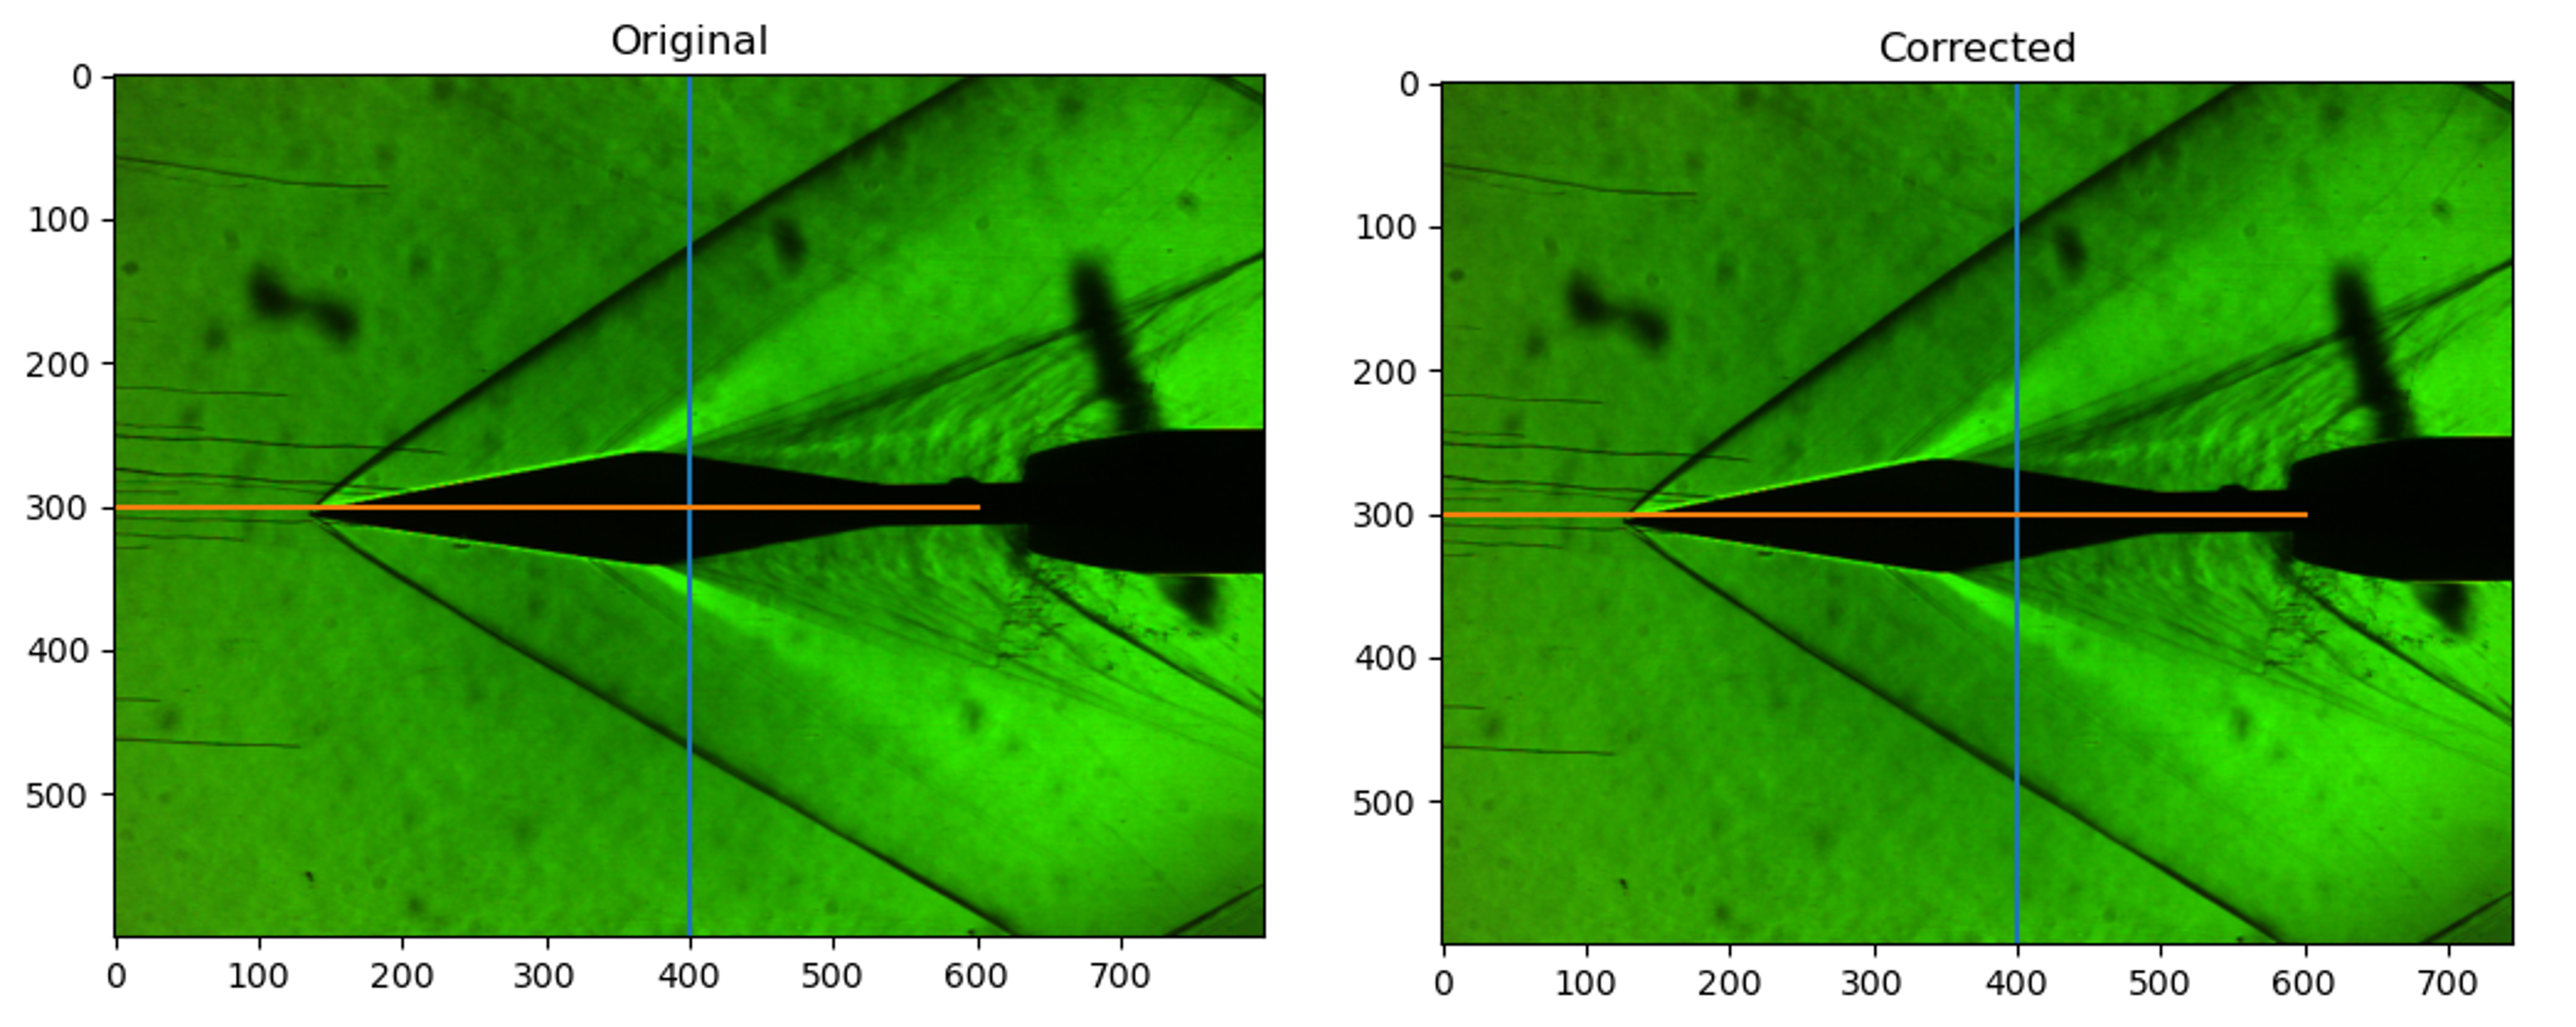
\includegraphics[width = \linewidth]{CorrectedImages/Diamond_AoA0_Mach25_corrected_vs_original.png}
    \caption{Corrected Example with Mach 2.5 flow at $0\degree$ angle of attack, Raw vs Corrected}
    \label{fig:correctionexample}
\end{figure}

\pagebreak

\subsection{True Mach \& Experimental vs Theoretical Surface Pressures}

The experimental surface pressures showed notable deviations from theoretical predictions across all test cases. When comparing the measured pressures to those calculated using shock-expansion theory with the true Mach numbers (derived from stagnation and static pressure measurements), several key discrepancies emerged:

\begin{itemize}
    \item The experimental pressures were consistently higher than theoretical predictions on the forward surfaces (P1 and P4)
    \item Pressure readings on the aft surfaces (P2 and P3) showed lower values than theory predicted
    \item These differences became more pronounced at higher angles of attack
\end{itemize}

These discrepancies can be attributed to several factors:

\begin{enumerate}
    \item \textbf{Non-ideal Geometry}: The test article is subscale, which causes the shock waves and expansion fans to form differently than predicted due to scaling boundary layer effects.
    
    \item \textbf{Boundary Layer Effects}: The presence of boundary layers, particularly at the leading edge, effectively changes the body shape the flow sees, altering the pressure distribution.
    
    \item \textbf{Flow Non-uniformity}: Small variations in the freestream conditions and potential flow angularity in the test section could contribute to asymmetric pressure distributions.
    
    \item \textbf{Measurement Uncertainty}: As detailed in the uncertainty analysis, the pressure measurements carry significant uncertainty, particularly at higher Mach numbers.
\end{enumerate}

\subsubsection{Pressure Transducer Uncertainty Analysis}


The resolution is determined by the digitization of the analog signal:

$$
\text{Resolution} = \text{Slope} \cdot \frac{\text{Steps}}{\text{Full Scale Voltage}}
$$

where:
\begin{enumerate}
    \item Steps = $2^{\text{Bits}} = 2^{12} = 4096$
    \item Full Scale Voltage = 0.5V
    \item Step size = $\frac{\text{Steps}}{\text{Full Scale Voltage}} = 1\text{e-}4$
\end{enumerate}


Static Pressure ($\approx 60 psi$) Individual Error Components

$$
\begin{aligned}
\text{Resolution} &= 0.0183 \text{ psi} = 0.3947 \text{ kPa} \\
\text{Linearity} &= 60 \text{ psi} \cdot 0.0025 = 0.15 \text{ psi} \\
\text{Repeatability} &= 60 \text{ psi} \cdot 0.002 = 0.12 \text{ psi} \\
\text{Temperature Shift} &= 60 \text{ psi} \cdot 0.0075 = 0.45 \text{ psi} \\
\text{Null Shift} &= 60 \text{ psi} \cdot 0.005 = 0.3 \text{ psi}
\end{aligned}
$$

Stagnation Pressure ($\approx 300 psi$)

Individual Error Components
$$
\begin{aligned}
\text{Resolution} &= 0.0732 \text{ psi} = 1.579 \text{ kPa} \\
\text{Linearity} &= 300 \text{ psi} \cdot 0.0025 = 0.75 \text{ psi} \\
\text{Repeatability} &= 300 \text{ psi} \cdot 0.002 = 0.6 \text{ psi} \\
\text{Temperature Shift} &= 300 \text{ psi} \cdot 0.075 = 2.25 \text{ psi} \\
\text{Null Shift} &= 300 \text{ psi} \cdot 0.005 = 1.5 \text{ psi}
\end{aligned}
$$

The total uncertainty is calculated using the Root Mean Square (RMS) method, combining all individual error components:

$$
u_{\text{RMS}} = \sqrt{u_1^2 + u_2^2 + ... + u_n^2}
$$

where $u_i$ represents each individual uncertainty component.

$$
u_{\text{Total}} = \sqrt{\text{Resolution}^2 + \text{Linearity}^2 + \text{Repeatability}^2 + \text{Temperature Shift}^2 + \text{Null Shift}^2}
$$

$$
\begin{aligned}
\text{Static Pressure Uncertainty} &= \pm 0.81 \text{ psi} \\
\text{Stagnation Pressure Uncertainty} &= \pm 4.06 \text{ psi}
\end{aligned}
$$

\begin{enumerate}
    \item All measurements are based on a full scale voltage of 0.5V.
    \item 12-bit analog-to-digital conversion is used (4096 steps).
    \item Uncertainty components are manufacturer-specified percentages of full scale.
    \item Temperature and null shift effects are included in the total uncertainty calculation.
\end{enumerate}

\subsubsection{Mach Number \& Aerodynamic Coefficient Uncertainty Analysis}

The Mach number is determined using the ratio of stagnation to static pressure:

$$M = \sqrt{\frac{2}{\gamma-1}\left[\left(\frac{P_0}{P}\right)^{\frac{\gamma-1}{\gamma}} - 1\right]}$$

\noindent where:
\begin{enumerate}
    \item $P_0$ is the stagnation pressure
    \item $P$ is the static pressure
    \item $\gamma$ is the specific heat ratio (1.4 for air)
\end{enumerate}

\noindent Individual Error Components for Mach Number:
$$
\begin{aligned}
\text{Stagnation Pressure Term} &= \frac{\partial M}{\partial P_0}\Delta P_0 = \pm 4.06 \text{ psi} \\
\text{Static Pressure Term} &= \frac{\partial M}{\partial P}\Delta P = \pm 0.81 \text{ psi}
\end{aligned}
$$

The total uncertainty is calculated using the Root Mean Square (RMS) method:

$$u_M = \sqrt{\left(\frac{\partial M}{\partial P_0}\Delta P_0\right)^2 + \left(\frac{\partial M}{\partial P}\Delta P\right)^2}$$

\vspace{5mm}

\noindent For the lift coefficient:

$$C_l = \frac{1}{\gamma P_{\infty} M_{\infty}^2 \cos{(\theta)}} [(P_3 - P_2)\cos{(\theta + \alpha)} + (P_4-P_1)\cos{(\theta-\alpha)}]$$

\noindent Individual Error Components
$$
\begin{aligned}
\text{P}_1 \text{ Term} &= \frac{\partial C_l}{\partial P_1}\Delta P_1 = \pm 0.81 \text{ psi} \\
\text{P}_2 \text{ Term} &= \frac{\partial C_l}{\partial P_2}\Delta P_2 = \pm 0.81 \text{ psi} \\
\text{P}_3 \text{ Term} &= \frac{\partial C_l}{\partial P_3}\Delta P_3 = \pm 0.81 \text{ psi} \\
\text{P}_4 \text{ Term} &= \frac{\partial C_l}{\partial P_4}\Delta P_4 = \pm 0.81 \text{ psi} \\
\text{Mach Term} &= \frac{\partial C_l}{\partial M_{\infty}}\Delta M_{\infty} = -\frac{2C_l}{M_{\infty}}u_M
\end{aligned}
$$

\vspace{5mm}

\noindent For the drag coefficient:

$$C_d = \frac{1}{\gamma P_{\infty} M_{\infty}^2 \cos{(\theta)}} [(P_1 - P_4)\sin{(\theta - \alpha)} + (P_3 - P_2)\sin{(\theta + \alpha)}]$$

\noindent Individual Error Components
$$
\begin{aligned}
\text{P}_1 \text{ Term} &= \frac{\partial C_d}{\partial P_1}\Delta P_1 = \pm 0.81 \text{ psi} \\
\text{P}_2 \text{ Term} &= \frac{\partial C_d}{\partial P_2}\Delta P_2 = \pm 0.81 \text{ psi} \\
\text{P}_3 \text{ Term} &= \frac{\partial C_d}{\partial P_3}\Delta P_3 = \pm 0.81 \text{ psi} \\
\text{P}_4 \text{ Term} &= \frac{\partial C_d}{\partial P_4}\Delta P_4 = \pm 0.81 \text{ psi} \\
\text{Mach Term} &= \frac{\partial C_d}{\partial M_{\infty}}\Delta M_{\infty} = -\frac{2C_d}{M_{\infty}}u_M
\end{aligned}
$$

\vspace{5mm}

\noindent For the center of pressure (at $\alpha = 0\degree$):

$$\frac{CP_x}{c} = \frac{\frac{1}{4}P_1 + \frac{3}{4}P_2}{P_1 + P_2}$$

\noindent Individual Error Components
$$
\begin{aligned}
\text{P}_1 \text{ Term} &= \frac{\partial (CP_x/c)}{\partial P_1}\Delta P_1 = \pm 0.81 \text{ psi} \\
\text{P}_2 \text{ Term} &= \frac{\partial (CP_x/c)}{\partial P_2}\Delta P_2 = \pm 0.81 \text{ psi}
\end{aligned}
$$

\noindent For y-direction center of pressure:

$$\frac{CP_y}{t} = \frac{P_1 - P_2 - P_3 + P_4}{2(P_1 - P_2 + P_3 - P_4)}$$

\noindent Individual Error Components
$$
\begin{aligned}
\text{P}_1 \text{ Term} &= \frac{\partial (CP_y/t)}{\partial P_1}\Delta P_1 = \pm 0.81 \text{ psi} \\
\text{P}_2 \text{ Term} &= \frac{\partial (CP_y/t)}{\partial P_2}\Delta P_2 = \pm 0.81 \text{ psi} \\
\text{P}_3 \text{ Term} &= \frac{\partial (CP_y/t)}{\partial P_3}\Delta P_3 = \pm 0.81 \text{ psi} \\
\text{P}_4 \text{ Term} &= \frac{\partial (CP_y/t)}{\partial P_4}\Delta P_4 = \pm 0.81 \text{ psi}
\end{aligned}
$$

The total uncertainty for each coefficient is calculated using the Root Mean Square (RMS) method:

$$u_{\text{Total}} = \sqrt{\sum_{i=1}^n u_i^2}$$

\noindent where $u_i$ represents each individual uncertainty component.

\begin{enumerate}
    \item All pressure measurements use the uncertainties determined in the pressure transducer analysis
    \item Mach number uncertainty is propagated through the coefficient calculations
    \item Angular uncertainties in $\alpha$ and $\theta$ are assumed negligible compared to pressure uncertainties
    \item Temperature effects are included through the pressure uncertainties
    \item Partial derivatives are evaluated at the measured conditions
\end{enumerate}

\subsection{Data Plots}

The experimental data revealed several interesting trends when examining $C_D$ vs. Mach number, $C_L$ vs. angle of attack, and $C_D$ vs. $C_L$:

\begin{figure}[H]
    \centering
    \includegraphics[width=\linewidth]{OtherPlots/CdvM_AoA0.png}
    \caption{$C_D$ vs Mach at $\alpha = 0^\circ$}
    \label{fig:cd_vs_mach_0}
\end{figure}

\begin{figure}[H]
    \centering
    \includegraphics[width=\linewidth]{OtherPlots/CdvM_AoA3.png}
    \caption{$C_D$ vs Mach at $\alpha = 3^\circ$}
    \label{fig:cd_vs_mach_3}
\end{figure}

\begin{figure}[H]
    \centering
    \includegraphics[width=\linewidth]{OtherPlots/CdvM_AoA7.png}
    \caption{$C_D$ vs Mach at $\alpha = 7^\circ$}
    \label{fig:cd_vs_mach_7}
\end{figure}

\begin{itemize}
    \item \textbf{$C_D$ vs. Mach}: The drag coefficient showed a general decrease with increasing Mach number, though not as pronounced as theory predicts. This trend aligns with the expected behavior as shock wave angles become more oblique at higher Mach numbers.
\end{itemize}

\begin{figure}[H]
    \centering
    \includegraphics[width=0.8\linewidth]{OtherPlots/CdvM_TheoryvsMeas.png}
    \caption{Drag coefficient vs Mach number comparison between theory and experiment}
    \label{fig:cd_vs_mach-theoryvmeas}
\end{figure}

\begin{itemize}    
    \item \textbf{$C_L$ vs. AoA}: The lift coefficient increased nearly linearly with angle of attack, but with a lower slope than theoretical predictions. This suggests reduced lift effectiveness, likely due to the blunted leading edge and flow separation effects.
\end{itemize}

\begin{figure}[H]
    \centering
    \includegraphics[width=0.8\linewidth]{OtherPlots/dragpolar_theoryvmeas.png}
    \caption{Drag polar comparison between theory and experiment}
    \label{fig:drag_polar-theoryvmeas}
\end{figure}

\begin{itemize}
    \item \textbf{$C_D$ vs. $C_L$}: The drag polar showed higher minimum drag and a steeper increase in drag with lift compared to theoretical predictions, indicating increased form drag and possibly earlier flow separation.
\end{itemize}

\subsection{Theoretical Plots}

Comparing the experimental results to linearized supersonic potential theory reveals significant insights:

The theoretical predictions for lift and drag coefficients:
\begin{equation*}
    C_L = \frac{4\alpha}{\sqrt{M_\infty^2 - 1}}
\end{equation*}

\begin{equation*}
    C_D = \frac{4\alpha^2 + 2\tan^2\theta}{\sqrt{M_\infty^2 - 1}}
\end{equation*}

The experimental results showed several deviations from these theoretical predictions:

\begin{itemize}
    \item The measured lift coefficients were consistently lower than theoretical values, particularly at higher angles of attack
    \item Drag coefficients exceeded theoretical predictions across all test conditions
    \item The relationship between $C_L$ and $\alpha$ showed less linearity than predicted
\end{itemize}

These discrepancies can be attributed to:
\begin{enumerate}
    \item Viscous effects not accounted for in the potential theory
    \item Real gas effects at higher Mach numbers
    \item The presence of boundary layers and flow separation
    \item Manufacturing imperfections in the test article
\end{enumerate}

\subsection{Center of Pressure}

The center of pressure location showed interesting behavior across the test conditions:

\begin{figure}[H]
    \centering
    \includegraphics[width=0.8\linewidth]{OtherPlots/Xcp_TheorvMeas.png}
    \caption{Center of pressure location comparison between theory and experiment}
    \label{fig:xcp-theoryvmeas}
\end{figure}

\begin{figure}[H]
    \centering
    \includegraphics[width=0.8\linewidth]{OtherPlots/Ycp_TheorvMeas.png}
    \caption{Vertical center of pressure location comparison between theory and experiment}
    \label{fig:ycp-theoryvmeas}
\end{figure}

\begin{itemize}
    \item For the symmetric case ($\alpha = 0^\circ$), the experimental center of pressure was located further forward than theory predicted
    \item With increasing angle of attack, the center of pressure showed more movement than theoretical calculations suggested
    \item The variation with Mach number was more pronounced in experimental results
\end{itemize}

This behavior differs from subsonic airfoils, where the center of pressure typically moves forward with increasing angle of attack. In our supersonic case, the center of pressure movement was more complex due to the interaction of shock waves and expansion fans.

The discrepancies between theoretical and experimental values can be attributed to:
\begin{enumerate}
    \item The non-ideal/subscale geometry of the test article affecting shock and expansion fan locations
    \item Boundary layer effects modifying the effective shape seen by the flow
    \item Measurement uncertainties in pressure readings affecting the moment calculations
    \item Flow separation effects at higher angles of attack
\end{enumerate}



\section{Conclusion}

The experimental investigation of supersonic flow over a diamond airfoil at Mach numbers 2.0-3.0 and angles of attack 0°-7° revealed both agreements with and deviations from shock-expansion theory. While fundamental behaviors such as decreasing shock angles with increasing Mach number were confirmed, several significant discrepancies were observed:

\begin{itemize}
    \item Expansion fans and recompression shocks occurred more upstream than theoretically predicted
    \item Measured drag coefficients exceeded theoretical predictions across all test conditions
    \item Lift coefficients were consistently lower than theoretical values, particularly at higher angles of attack
    \item Center of pressure locations showed greater variation with Mach number than theory suggested
    \item Pressure distributions deviated systematically, with higher pressures on forward surfaces and lower pressures on aft surfaces
\end{itemize}

These deviations can be attributed to physical phenomena not accounted for in shock-expansion theory:
\begin{itemize}
    \item Boundary layer effects modifying the effective body shape
    \item Viscous effects, particularly at the leading edge
    \item Flow separation at higher angles of attack
\end{itemize}

Significant measurement uncertainties (±0.81 psi for static pressure, ±4.06 psi for stagnation pressure) affected the calculated aerodynamic coefficients. Future experiments could benefit from sharper-edged test articles, more precise pressure measurements, and additional instrumentation for boundary layer characterization.

Despite these limitations, the experiment successfully demonstrated the fundamental physics of supersonic flow over a diamond airfoil and highlighted important practical limitations of theoretical predictions in supersonic aerodynamics.

\hypertarget{reference}{}
\section{References}

\begin{enumerate}
    \item Jernel, Lloyd  S. “Comparisons of Two-Dimensional Shock-Expansion Theory with Experimental Aerodynamic Data for Delta-Planform Wings at High Supersonic Speeds.” NASA, June 1, 1974. \url{https://ntrs.nasa.gov/citations/19740018331}. 
    \item Li, Sheng, Chen-Yuan Bai, and Zi-Niu Wu. “Nonlinear Supersonic Indicial Response of Diamond Airfoils.” Acta Mechanica 231, no. 6 (March 5, 2020): 2125-41. \url{https://doi.org/10.1007/s00707-020-02637-3}. 
    \item Wood, Richard M. “Supersonic Aerodynamics of Delta Wings.” NASA, March 1, 1988. \url{https://ntrs.nasa.gov/citations/19880008231}. 
    \item Serafini, John S. “Impingement of Water Droplets on Wedges and Diamond Airfoils at Supersonic Speeds.” NASA, July 1, 1953. \url{https://ntrs.nasa.gov/citations/19930083634}. 
    \item Holdaway, George, Jack Mellenthin, and Elaine Hatfield. “Investigation at Mach Numbers of 0.20 to 3.50 of a Blended Diamond Wing and Body Combination of Sonic Design but with Low Wave-Drag Increase with Increasing Mach Number.” NASA, October 1, 1959. \url{https://ntrs.nasa.gov/citations/19980232906}. 
    \item Heaslet, Max A., and Harvard Lomax. “Two-Dimensional Unsteady Lift Problems in Supersonic Flight.” NASA, January 1, 1949. \url{https://ntrs.nasa.gov/citations/19930092010}. 
\end{enumerate}

\pagebreak
\appendix
\pagenumbering{gobble} 
\begin{center}
\vspace*{\fill}
   \Huge \bf Appendix 
\vspace*{\fill}
\end{center}
\pagebreak 


\hypertarget{derivations}{}
\section{Derivations}

Equations for lift and drag analysis:

\begin{equation*}
    C_{l} = \dfrac{l}{\frac{1}{2}\rho_{\infty}U_{\infty}^{2}c} = \dfrac{l}{\frac{1}{2}\gamma P_{\infty} M_{\infty}^{2} c}
\end{equation*}
\vspace{5mm}

\begin{equation*}
    C_{d} = \dfrac{d}{\frac{1}{2}\rho_{\infty}U_{\infty}^{2}c} = \dfrac{d}{\frac{1}{2}\gamma P_{\infty} M_{\infty}^{2} c}
\end{equation*}
\vspace{5mm}

\begin{equation*}
    l = P_{3}z\cos{(\theta + \alpha)} + P_{4}z\cos{(\theta-\alpha)}-P_{1}z\cos{(\theta-\alpha)} - - P_{2}z\sin{(\theta + \alpha)}
\end{equation*}
\vspace{5mm}

\begin{equation*}
    d = P_{1}z\sin{(\theta - \alpha)} + P_{3}z\sin{(\theta + \alpha)} - P_{2}z\sin{(\theta + \alpha)} - P_{4}z\sin{(\theta - \alpha)}
\end{equation*}
\vspace{5mm}

\begin{equation*}
    C_{l} = \dfrac{z}{\frac{1}{2}\gamma P_{\infty} M_{\infty}^{2} c} \left[(P_{3} - P_{2})\cos{(\theta + \alpha)} + (P_{4}-P_{1})\cos{(\theta-\alpha)}\right]
\end{equation*}
\vspace{5mm}

\begin{equation*}
    C_{d} = \dfrac{z}{\frac{1}{2}\gamma P_{\infty} M_{\infty}^{2} c} \left[(P_{3} - P_{2})\sin{(\theta + \alpha)} + (P_{1} - P_{4})\sin{(\theta - \alpha)}\right]
\end{equation*}
\vspace{5mm}

\begin{equation*}
    z = \dfrac{(c/2)}{\cos{(\theta)}}
\end{equation*}
\vspace{5mm}

\begin{equation*}
    C_{l} = \dfrac{1}{\gamma P_{\infty} M_{\infty}^{2} \cos{(\theta)}} \left[(P_{3} - P_{2})\cos{(\theta + \alpha)} + (P_{4}-P_{1})\cos{(\theta-\alpha)}\right]
\end{equation*}
\vspace{5mm}

\begin{equation*}
    C_{d} = \dfrac{1}{\gamma P_{\infty} M_{\infty}^{2} \cos{(\theta)}} \left[(P_{1} - P_{4})\sin{(\theta - \alpha)} + (P_{3} - P_{2})\sin{(\theta + \alpha)}\right]
\end{equation*}
\vspace{5mm}

\end{document}